\chapter{Design of MPI\_T support in TAU}

\section {Design}
The existence of MPI\_T provides an opportunity to link together the components above. However, each component must be extended to interact through the MPI\_T interface, as well as in concert with each other. Below, we describe the design approach for MVAPICH2 and TAU integration to enable runtime introspection, performance tuning, and recommendation generation. Figure \ref{fig:mpitinfrastructure} depicts the infrastructure architecture and component interactions.
\subsection {Enhancing MPI\_T Support in MVAPICH2}
MVAPICH2 exports a wide range of performance and control variables \\ through the MPI\_T interface. A performance variable represents an internal metric or counter, and setting a control variable may alter the behavior of the library. Current support for MPI\_T variables in MVAPICH2 broadly fall under the following categories:
\subsubsection {Monitoring and Modifying Collective Algorithms} 
For collective operations such as \verb+MPI_Bcast+ and \verb+MPI_Allreduce+, there are a variety of algorithms available and the right algorithm to use depends on a number of parameters such as system metrics (bandwidth, latency), the number of processes communicating and the message size. MVAPICH2 exports CVARs that can be used to determine the collective algorithm based on the message size. It also supports PVARs that monitor the number of times a certain collective algorithm is invoked.
\begin{center}
	\begin{figure*}[tbp!]
         \centering
		%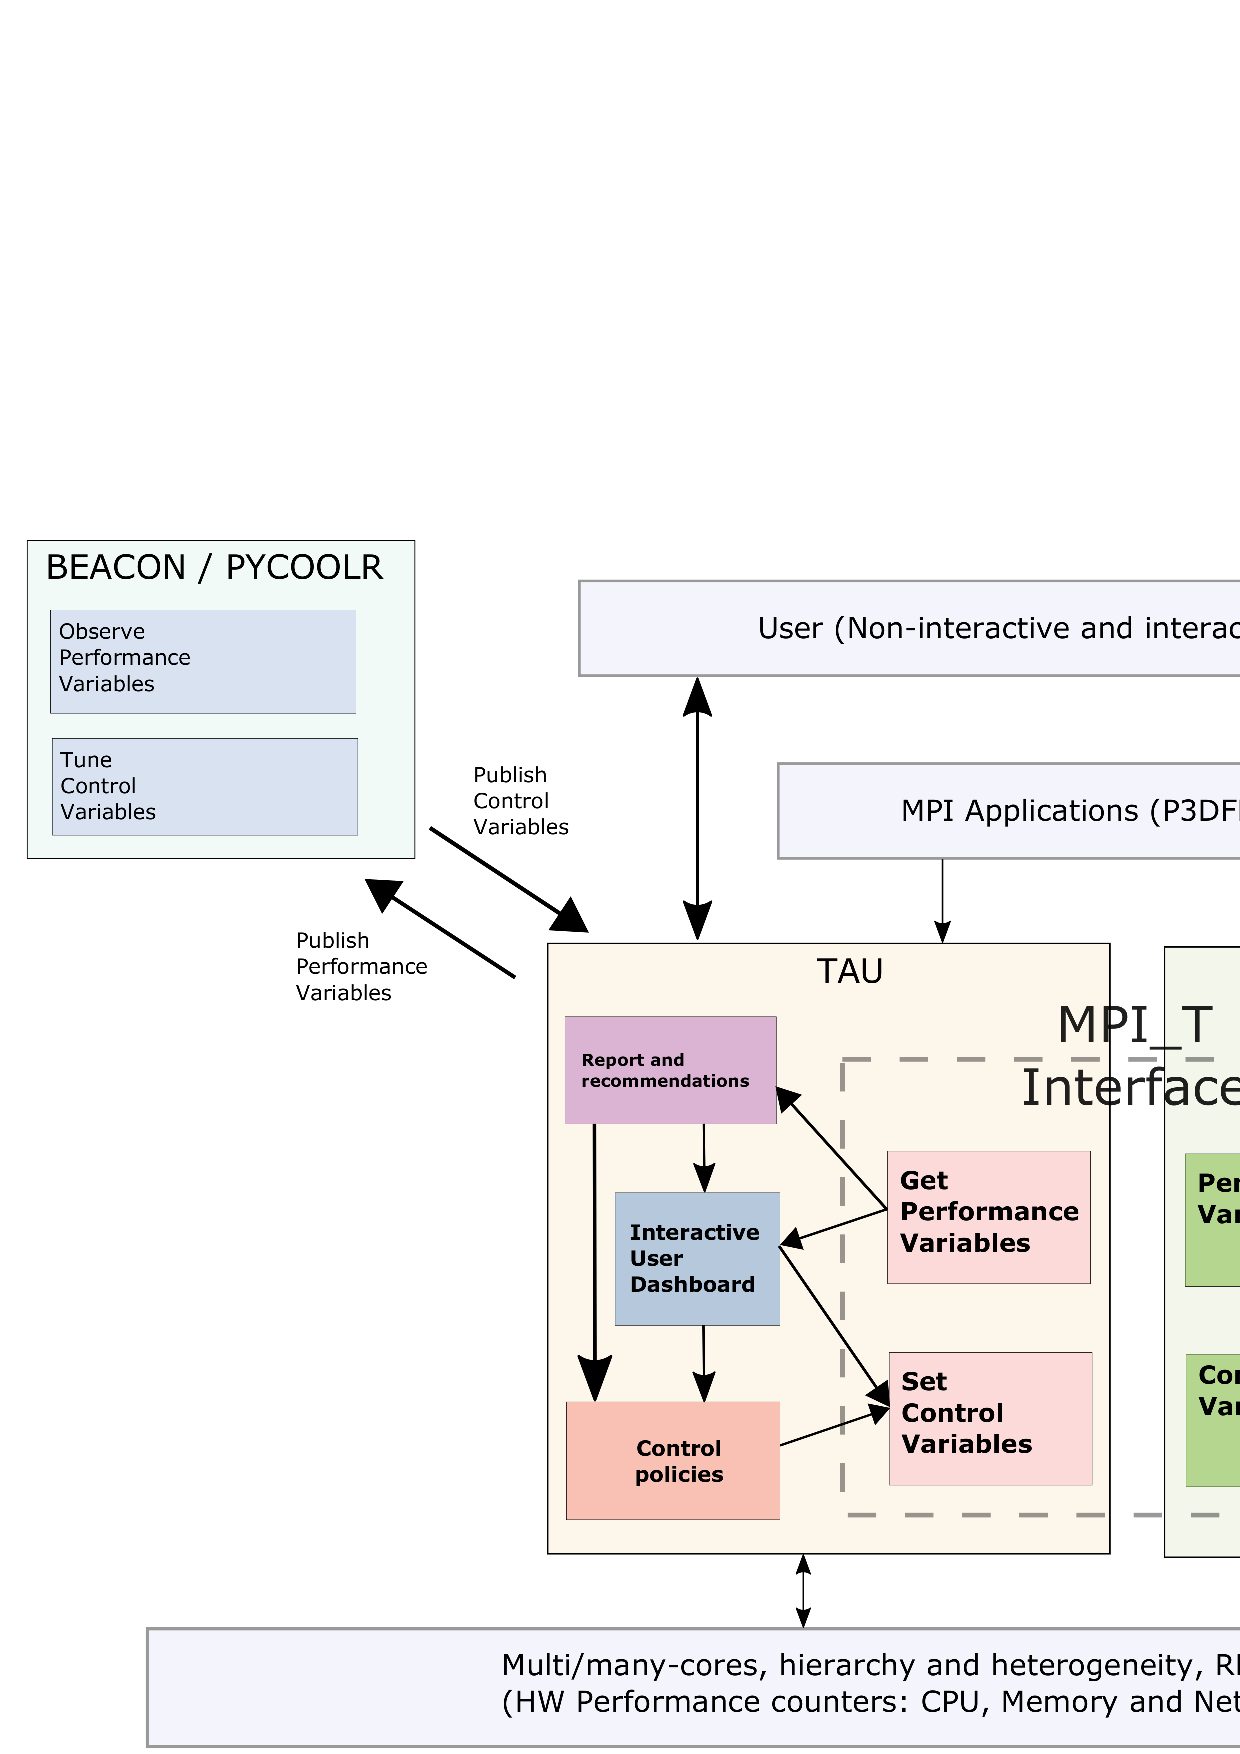
\includegraphics[width=\textwidth,scale=0.05]{figures/MPI_T_infrastructure}
		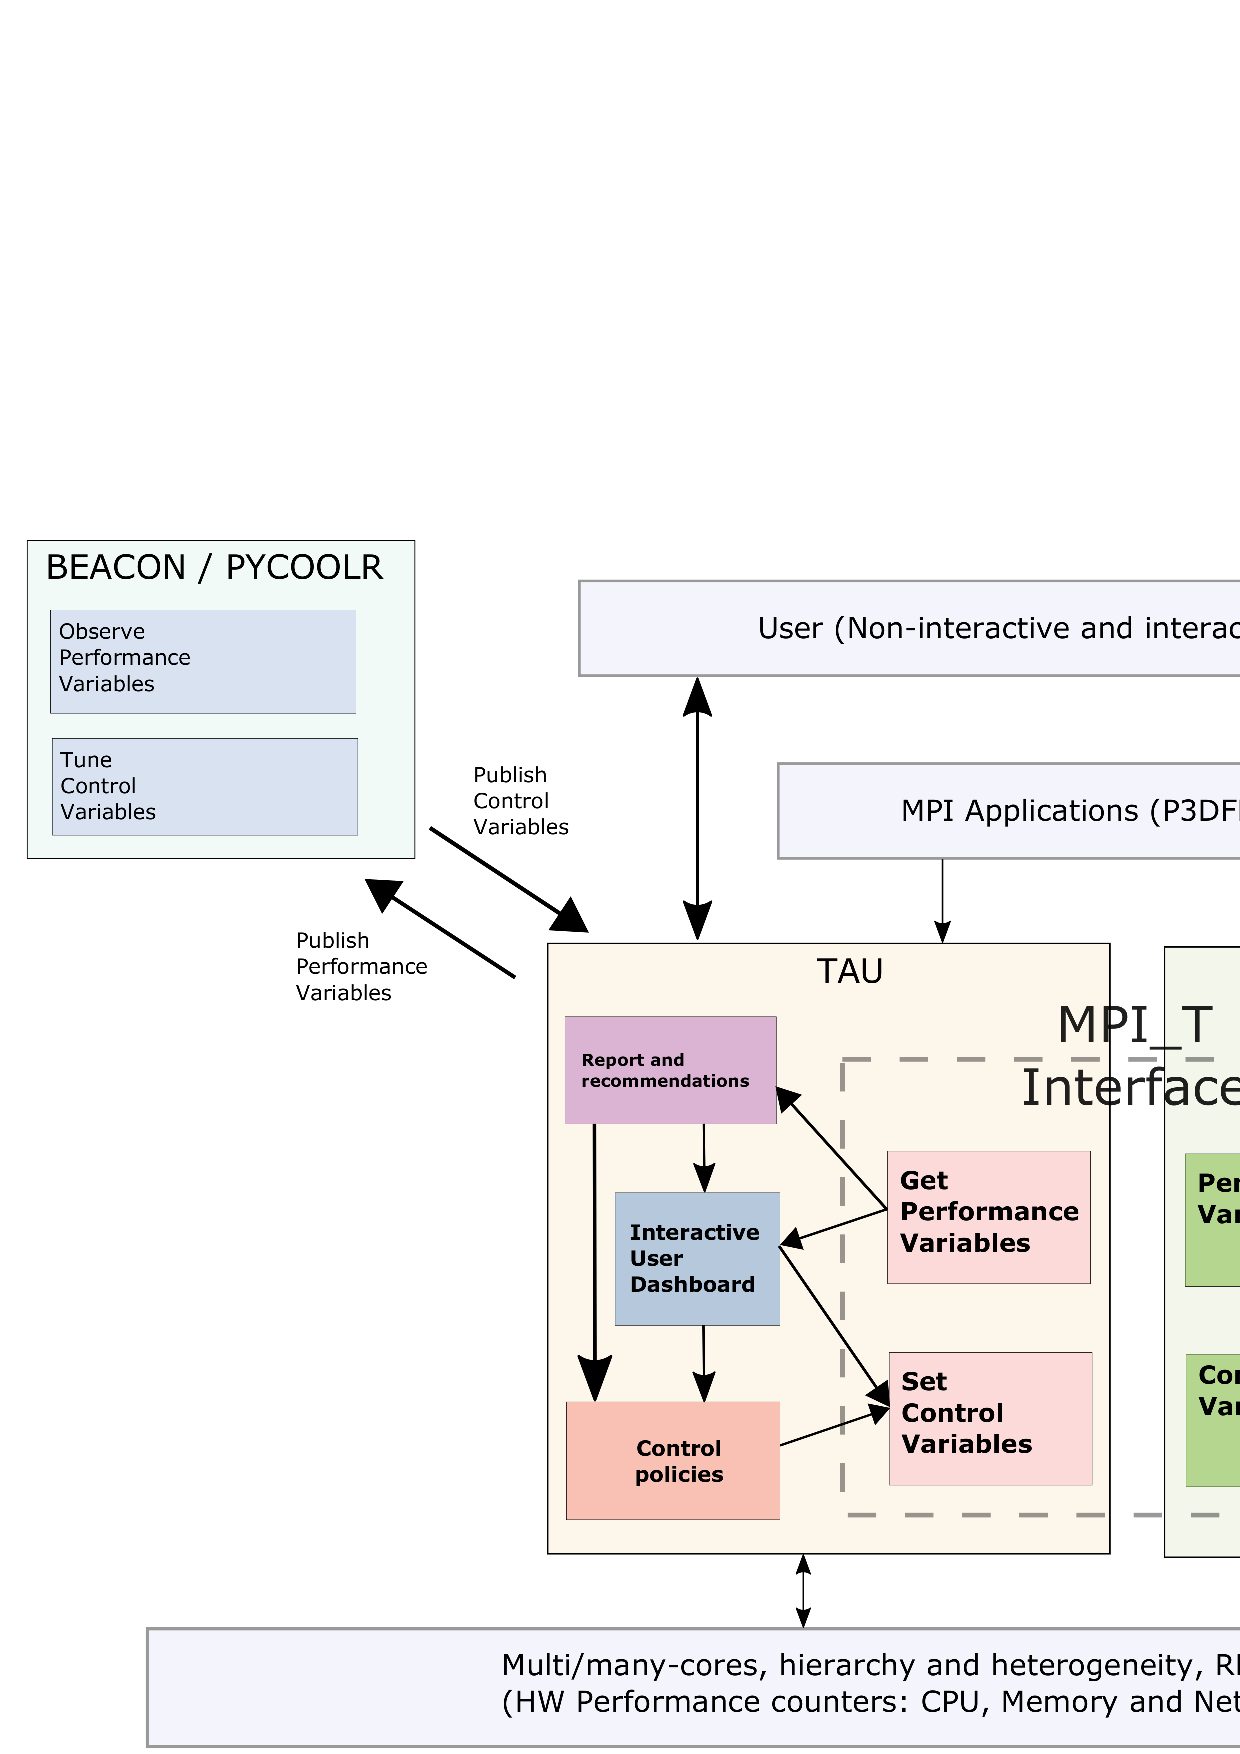
\includegraphics[scale=0.3, width=\columnwidth, keepaspectratio]{figures/MPI_T_infrastructure}
		\caption{Integrated MVAPICH2 and TAU infrastructure based on MPI\_T}
		\label{fig:mpitinfrastructure}
	\end{figure*}
\end{center}

\subsubsection {Monitoring and Controlling Usage of Virtual Buffers} 
Virtual Buffers (VBUFs) are used in MVAPICH2 to temporarily store messages in transit between two processes. The use of virtual buffers can offer significant performance improvement to applications performing heavy point-to-point communication, such as stencil-based codes. MVAPICH2 offers a number of PVARs that monitor the current usage level, availability of free VBUFs in different VBUF pools, maximum usage levels, and the number of allocated VBUFs at process level granularity. Accordingly, it exposes CVARs that modify how MVAPICH2 allocates and frees these VBUFs at runtime.

\subsection{Enabling Runtime Instrospection and Online Monitoring}
MPI\_T makes it possible to inquire about the state of the underlying MPI implementation through the query of performance variables. While it is the prerogative of the MPI implementation what PVARs are published, the tool must be extended to use MPI\_T for access. Similarly, control variables are defined by the MPI implementation but set by the tool using MPI\_T. Below we discuss how this is done in TAU to realize introspection and tuning.
\subsubsection{Gathering Performance Data}
TAU has been extended to support the gathering of performance data exposed through the MPI\_T interface. Each tool that is interested in querying MPI\_T must first register a \textit{performance session} with the interface. This object allows the MPI library to store separate contexts and differentiate between multiple tools/components that are simultaneously querying the MPI\_T interface. Along with a \textit{performance session}, a tool must also allocate \textit{handles} for all the performance variables that it wishes to read/write. Within TAU, the task of allocating the global (per-process) performance session and handles for PVARs is carried out inside the TAU tool initialization routine. However, this design has a caveat --- an MPI library can export additional PVARs during runtime as they become available through dynamic loading. A tool must accordingly allocate handles for these additional PVARs if it wishes to read them. TAU currently does not support this --- we are restricted to reading PVARs that are exported at TAU initialization. We plan to support the dynamic use case in a future release.
\par TAU can use sampling to collect performance variables periodically. When an application is profiled with TAU's MPI\_T capabilities enabled, an interrupt is triggered at regular intervals. Inside the signal handler for the \verb+SIGUSR+ signal, the MPI\_T interface is queried and the values of \textit{all} the performance variables exported are stored at process level granularity. TAU registers internal \textit{atomic user events} for each of these performance variables, and every time an event is triggered (while querying the MPI\_T interface), the running average, minimum value, the maximum value, and other basic statistics are calculated and available to the user at the end of the profiling run. These statistics carry meaning only for PVARs that represent \verb+COUNTERS+ or \verb+TIMERS+. Thus, we define TAU user events to store and analyze PVARs for these two classes. The MPI\_T interface allows MPI libraries to export PVARs from a rich variety of classes --- timers, counters, watermarks, state information, etc. MVAPICH2 and TAU have been primarily designed to support PVARs from the \verb+TIMER+ or \verb+COUNTER+ classes. As part of future work, we plan to export a richer variety of PVAR classes and design appropriate methods for storage and analysis of each of these classes.

\subsubsection{Online Monitoring}
Runtime introspection naturally extends to online monitoring where certain performance variables are made viewable during execution. Figure \ref{fig:onlinemonitoringdesign} depicts the interaction between TAU and BEACON to enable online monitoring of PVARs through the PYCOOLR GUI.
\par To interface TAU and BEACON, TAU defines a BEACON \textit{topic} for performance variables and publishes PVAR data collected at runtime to this topic. Any software component interested in monitoring PVARs can then subscribe to this topic and receive live updates for all performance variables exported by the MPI implementation.
\par To monitor PVARs on PYCOOLR, the PYCOOLR GUI acts as a subscriber to the PVAR topic --- thus it receives updated values for all PVARs from TAU's sampling based measurement module. The GUI has been extended to offer the user the ability to select only those PVARs that he/she is interested in monitoring --- this is a useful feature as an MPI library can export 100's of PVARs, not all of which may interest the user. The GUI plots the values for the selected PVARs at runtime as and when it receives them through BEACON.

\subsubsection{Viewing Performance Data}
ParaProf is the TAU component that allows the user to view and analyze the collected performance profile data post-execution. This profile information is collected on a per-thread or a per-process level, depending on whether or not threads were used in the application. ParaProf has existing support for the analysis of \textit{interval events} as well as \textit{atomic user events}. Interval events are used to capture information such as the total execution time spent inside various application routines. Atomic user events are used to store information such as hardware counter values. 
\par As described in Section 5.2.1, PVARs are treated as atomic user events. ParaProf's existing support for analyzing atomic user events has been leveraged to display PVAR data for each process. Performance variables collected from the MPI\_T interface during execution are displayed on \verb+ParaProf+ as events that include markers indicating high variability.

\begin{center}
        \begin{figure*}[tbp!]
        \centering
                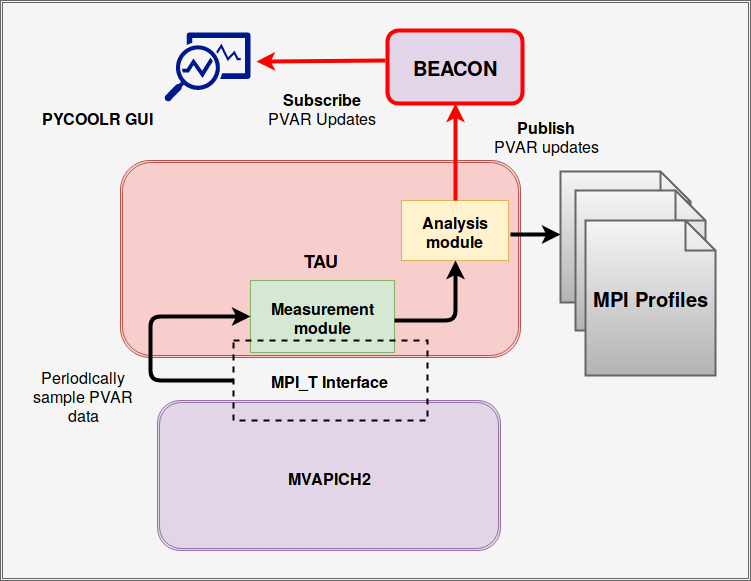
\includegraphics[scale=0.35,keepaspectratio]{figures/Online_Monitoring_Design}
                \caption{Online Monitoring with BEACON/PYCOOLR}
                \label{fig:onlinemonitoringdesign}
        \end{figure*}
\end{center}

\subsection{Runtime Tuning through MPI\_T}
Complementary to providing an API for runtime introspection, the MPI\_T interface also enables a mechanism to modify the behavior of the MPI library through control variables. MPI implementations can define control variables for configuration, performance, or debugging purposes. MPI libraries may implicitly restrict the semantics of \textit{when} CVARs can be set --- some may be set only once before \verb+MPI_Init+, and others may be set anytime during execution. Further, there may be restrictions on whether or not CVARs are allowed to have different values for different processes --- this decision is left entirely up to the MPI library. Therefore, a tool or a user interacting with the MPI\_T interface for the purpose of tuning the MPI library must be aware of the particular semantics associated with the CVARs of interest.
\subsubsection {User-Guided Tuning through PYCOOLR} Our infrastructure provides users the ability to fine-tune the MPI library by setting CVARs at runtime. As depicted in Figure \ref{fig:manualtuning}, we use the BEACON backplane communication infrastructure to enable user-guided tuning. TAU and BEACON interface with each other in a bi-directional fashion. Aside from acting as a publisher of PVAR data, TAU is a subscriber to a BEACON topic used for communicating CVAR updates. The PYCOOLR GUI has been extended to enable the user to set new values for multiple CVARs at runtime --- Figure \ref{fig:pycoolrcvars} displays a screenshot of the PYCOOLR window that enables this functionality.
\par Together with the online monitoring support provided by PYCOOLR, this user-guided tuning infrastructure can enable a user to experiment with different settings for CVARs and note their effects on selected PVARs or other performance metrics. We must note that this infrastructure has one significant limitation --- the value that the user sets for a CVAR is \textit{uniformly} applied across MPI processes. In other words, each MPI process receives the same value for the CVAR --- this may not be ideal, as it is likely that each process displays a different behavior and thus may have a different optimal value for a given setting. We argue that this infrastructure is nevertheless useful in the experimentation phase, wherein the user is trying to determine the CVAR that is important for a given situation/application.

\begin{center}
        \begin{figure*}[tbp!]
        \centering
                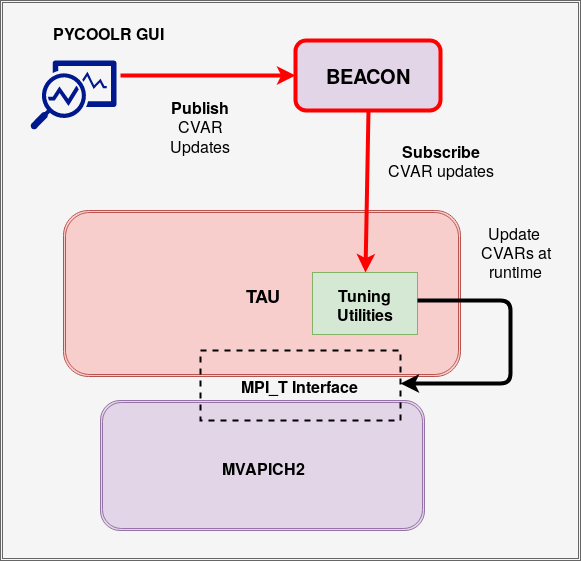
\includegraphics[scale=0.4,keepaspectratio]{figures/Manual_Tuning_Design}
                \caption{User-Guided Tuning with BEACON/PYCOOLR}
                \label{fig:manualtuning}
        \end{figure*}
\end{center}

\subsection{Plugin Infrastructure in TAU}

TAU is a comprehensive software suite that is comprised of well-separated components providing instrumentation, measurement and analysis capabilities. Our vision for performance engineering of MPI applications involves a \textit{more active} involvement of TAU in monitoring, debugging and tuning behavior \textit{at runtime}. The MPI\_T interface provides tools an opportunity to realize this vision.
\par Recall that the MPI\_T interface allows MPI implementations complete freedom in defining their own PVARs and CVARs to export. However, this freedom comes with a cost to tool writers for MPI\_T --- each MPI implementation will require its own custom tuning and re-configuration logic. From a software infrastructure development standpoint, it would be preferable to design a framework that will allow multiple such customized autotuning logic to co-exist \textit {outside of core tool logic}, and be appropriately loaded depending on the MPI library being used. With this motivation in mind, we have added support for a \textit{generic} plugin infrastructure in TAU that can be used to develop and load custom logic for a variety of performance engineering needs. The latest version of TAU\footnote{http://tau.uoregon.edu} supports this plugin infrastructure.

\begin{center}
        \begin{figure}[tbp!]
         \centering
         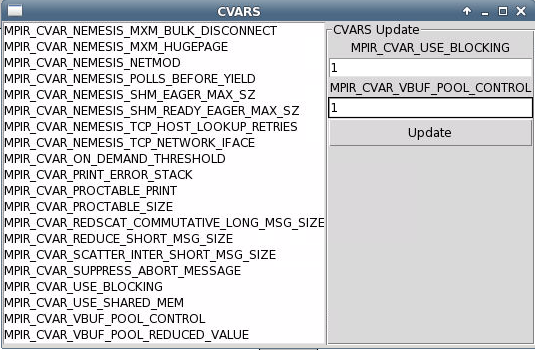
\includegraphics[scale=0.5,keepaspectratio]{figures/Pycoolr-CVARs}
         \caption{Screenshot of PYCOOLR window to update CVARs}
         \label{fig:pycoolrcvars}
        \end{figure}
\end{center}

\subsubsection{Design Overview} In the current design, plugins are \verb+C\+\verb+C+\texttt{++} modules that are built into separate shared libraries. The user can specify the path to the directory containing the plugins using the environment variable \verb+TAU_PLUGINS_PATH+. The user can also specify the plugins to be loaded using the environment variable \verb+TAU_PLUGINS+ separated by a delimiter. 
\par In keeping with the general design of plugin frameworks, the TAU plugin system has the following phases:
\begin {itemize}
\item \textbf{Initialization}: This is invoked during TAU library initialization. During this phase, TAU's plugin manager reads the environment variables \verb+TAU_PLUGINS_PATH+ and \verb+TAU_PLUGINS+ and loads the plugins in the order specified by \verb+TAU_PLUGINS+. Each plugin \textit{\textbf{must}} implement a function called \verb+Tau_plugin_init_func+. Inside this function, it can register callbacks for a subset of \textit{plugin events} it is interested in. Note that each plugin may register callbacks for more than one event. The plugin manager maintains an \textit{ordered} list of active plugins for each event supported.
\item \textbf{Event Callback Invocation}: We define some salient plugin events in TAU that could be interesting or useful from a performance engineering standpoint. These events are discussed in detail in Section 5.4.2. When these plugin events occur during execution of an application instrumented with TAU, the plugin manager invokes the registered callbacks for the specific event in the order in which the corresponding plugins were loaded. Each event that is supported has a specific, typed data object associated with it. When the event occurs, this data object is populated and sent as a parameter to the plugin callback. 
\item \textbf{Finalize Phase}: When TAU is done generating the profiles for the application, the plugins are unloaded, and all the auxiliary memory resources allocated by the plugin manager are freed.
\end{itemize}

\subsubsection{Plugin Events Supported}
Plugin events are entry points into the plugin code that performs a custom task. Currently, TAU defines and supports the following events:
\begin{itemize}
\item \verb+FUNCTION_REGISTRATION+: TAU creates and registers a \verb+FunctionInfo+ object for all functions it instruments and tracks. This event marks the end of the registration phase for the \verb+FunctionInfo+ object that was created.
\item \verb+ATOMIC_EVENT_REGISTRATION+: TAU defines \textit{atomic events} to track PAPI counters, PVARs and other entities which do not follow interval event semantics. This plugin event marks the end of the registration phase for the atomic event and is triggered when the atomic event is created. In the context of our MPI\_T infrastructure, this plugin event is triggered once for every PVAR that is exported by the MPI library.
\item \verb+ATOMIC_EVENT_TRIGGER+: When the value of an atomic event is updated, this event is triggered. This plugin event is triggered once for each PVAR, every time the MPI\_T interface is queried.
\item \verb+INTERRUPT_TRIGGER+: TAU's sampling subsystem relies on installing an interrupt handler for the \verb+SIGUSR+ signal, and performs the sampling within this interrupt handler. When TAU is used with its sampling capabilities turned on, this plugin event is triggered within TAU's interrupt handler (10 seconds is the default interrupt interval).
\item \verb+END_OF_EXECUTION+: When TAU has finished creating and writing the profile files for the application, this plugin event is triggered.
\end{itemize}
We plan to add to the list of supported events in future releases.

\subsubsection{Use Case: Filter Plugin to Disable Instrumentation at Runtime}
To demonstrate a sample usage scenario for the plugin architecture, we have created a plugin that filters out instrumented functions from being profiled at runtime, based on a user-provided selective instrumentation file. This situation arises when the application has been instrumented using either the compiler or TAU's source instrumentation tool --- the Program Database Toolkit (PDT)~\cite{PDT}.
\par PDT works by parsing the input source file to detect function definitions and function call sites, and automatically adds the TAU instrumentation API calls to these sites. The user may want to prevent certain \textit{automatically instrumented functions} from being profiled --- these functions may be frequently invoked but not have a significant impact on overall runtime. They may pollute the generated profiles and more importantly, add to the measurement overheads without providing any real benefit. From a profiling standpoint, there is solid motivation to provide a mechanism that allows such functions to be excluded from profiling.
\par We use our plugin infrastructure to provide this functionality --- our filter plugin registers a callback for the \verb+FUNCTION_REGISTRATION+ plugin event. Recall that this event is triggered once for every function instrumented by TAU. Within the callback for the \verb+FUNCTION_REGISTRATION+ event, we read a user-provided selective instrumentation file that contains a list of functions to be excluded from profiling. The data object for this plugin event contains the function name information. If there is a match between the function being registered and the list of function names in the selective instrumentation file, we set the profile group for the function to be \verb+TAU_DISABLE+, effectively switching off profiling for this function.
\subsection{Plugins for Autotuning}
Figure \ref{fig:plugininfrastructure} depicts TAU plugins in the context of our MPI\_T infrastructure. As discussed in Section 5.2, TAU samples PVAR data from the MPI\_T interface inside a signal handler for the \verb+SIGUSR+ signal. TAU can use this collected PVAR data to perform an autotuning decision inside the signal handler --- this is realized through plugins that install callbacks for the \verb+INTERRUPT_TRIGGER+ event. This event is triggered every time TAU samples the MPI\_T interface, and the registered plugin callbacks are invoked. Inside the callback, the plugin has access to all the PVAR data collected and performs a \textit{runtime autotuning decision} that may result in updated values for \textit{one or more} CVARs (knobs). Plugins can make use of core TAU modules to interact with the MPI\_T interface to update CVAR values.
\par Note that the plugin infrastructure allows the user to specify more than one plugin --- this feature can be utilized to load multiple autotuning policies, each of which is built into a separate shared library. While plugins use common functionality defined inside TAU to read or write to the MPI\_T interface, the autotuning logic itself is custom to each plugin --- in the future, we plan to support a high-level infrastructure to express autotuning policies that reduce duplicated code across plugins. Our starting point for developing autotuning policies relies on users with background or offline knowledge about specific domains, applications, and libraries.

\begin{center}
        \begin{figure*}[tbp!]
         \centering
                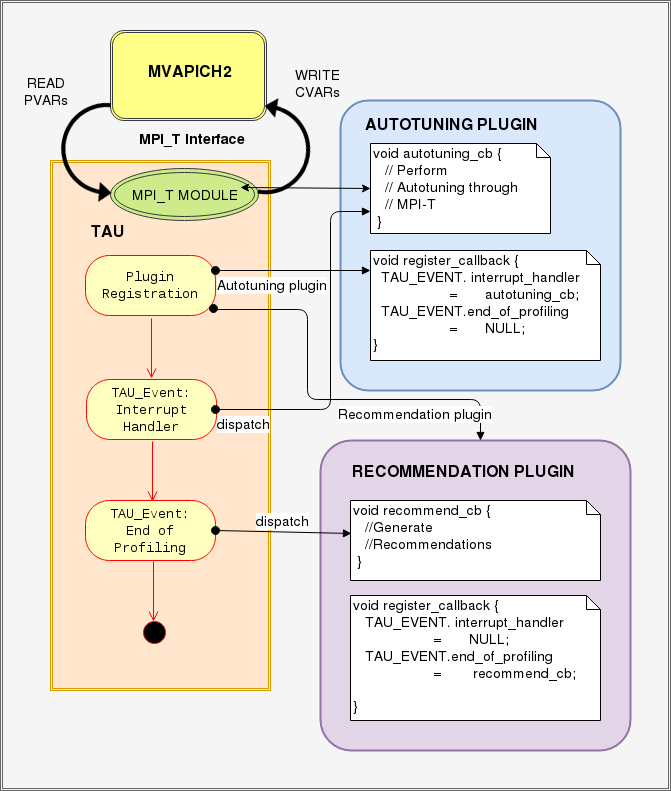
\includegraphics[scale=0.5,width=\columnwidth,keepaspectratio]{figures/Plugin_Infrastructure}
                \caption{Plugin Infrastructure}
                \label{fig:plugininfrastructure}
        \end{figure*}
\end{center}

\subsection{Plugins for Recommendations}
We take advantage of the plugin mechanism to develop performance recommendations for the user. MPI libraries can export a large number of control variables --- many of which are also environment variables whose default settings may not always be optimal for a given application/situation. Moreover, the user may not even be aware of the existence of certain settings or MPI implementation-specific features that can improve performance. A profiling tool such as TAU is in an ideal position to fill this gap with the MPI\_T interface acting as an enabling mechanism. \par Performance data gathered by TAU through the MPI\_T and PMPI interface can be analyzed by a recommendation plugin to provide useful hints to the user at the end of the application execution. Recommendation plugins register callbacks for the \verb+END_OF_EXECUTION+ event that is triggered when TAU has finished collecting and writing profile information. Currently, TAU supports the generation of recommendations as part of the metadata that is associated with each process. This metadata is available for viewing on \verb+ParaProf+.

